% Setup
\graphicspath{./figures}

\chapter{Background}
\label{chap:background}

% Introduction
% - Did not exist 10 years ago
% - Why now

A decade ago, \gls{sm} technology did not exist, at least not in its current form. It is a by-product of the evolution in application architectures and the trends in cloud-native application design \cite{balalaie2016microservices}. The shift to service-based architectural styles became popular when the \gls{devops} movement gained traction and became standard in the industry \cite{microservices-trends} Although this shift improved the speed and agility of software development \cite{amaral2015performance} it came at the cost of additional operational complexity and overheads which \glspl{sm} try to solve. 


The remainder of this chapter introduces several concepts and related topics relevant to this thesis. The topics are introduced in a specific order, which paints a general picture of the evolution and progression of technologies in the landscape. First, we introduce the concept of container technologies and talk about the mass adoption caused by \gls{docker} (\cref{sec:background:containers}). Secondly, we introduce the concept of \glspl{micro-service} as a natural evolution of the \gls{soa} architecture paradigm and how it is further enabled by the adoption of container technologies (\cref{sec:background:soa}). Furthermore, we introduce \gls{k8s}, the defacto standard in container orchestration and which problems it tries to solve (\cref{sec:background:kubernetes}). Finally, we go into the details of \gls{sm} technology where we introduce the core characteristics that define such a system and what problems this additional layer of networking abstraction tries to solve (\cref{sec:background:service-mesh}).

\missingfigure[figwidth=\textwidth]{Evolution of technologies in the landscape}


% Sections
\section{Containers}
\label{sec:background:containers}


% General introduction Container
A \gls{container} is a unit of executable software that is packaged with all of its dependencies \cite{docker-what-is-container, ibm-what-is-container}. By packaging everything in a single unit it makes it easy to run the application on different environments, from desktops and laptops to cloud environments. \Glspl{container} isolate software from their environment and ensure that it works uniformly on all devices regardless of operating systems used or the hardware powering it. 




% How it works
\Glspl{container} leverage a set of Linux technologies, such as \textit{cgroups} and \textit{namespaces}. The former is a mechanism to organize processes in hierarchical groups whose usage of various system resources can then be limited and monitored \cite{cgroups, man-cgroups}. The latter is a technology to wrap a system resource in an abstraction to make it appear to a process as if they had their own isolated instance of that resource \cite{man-namespaces}. These combined with the fact that a container has a layered file system that contains the application code and operating system dependencies makes it so that it is a fast and lightweight unit of compute. 

A comparison with \glspl{vm} is commonly made because of their isolating properties and abstractions. However, a \gls{vm} is a software-based virtualization of an entire computer system, this includes the hardware, the entire operating system that runs on it in addition to the applications and binaries that it requires. A \gls{container} on the other hand is an abstraction at the application level, where it is simply just another process living in user space. A comparison of the different deployment models can be seen in \ref{fig:vm-vs-container}.


\begin{figure}[!t]
    \centering
    
    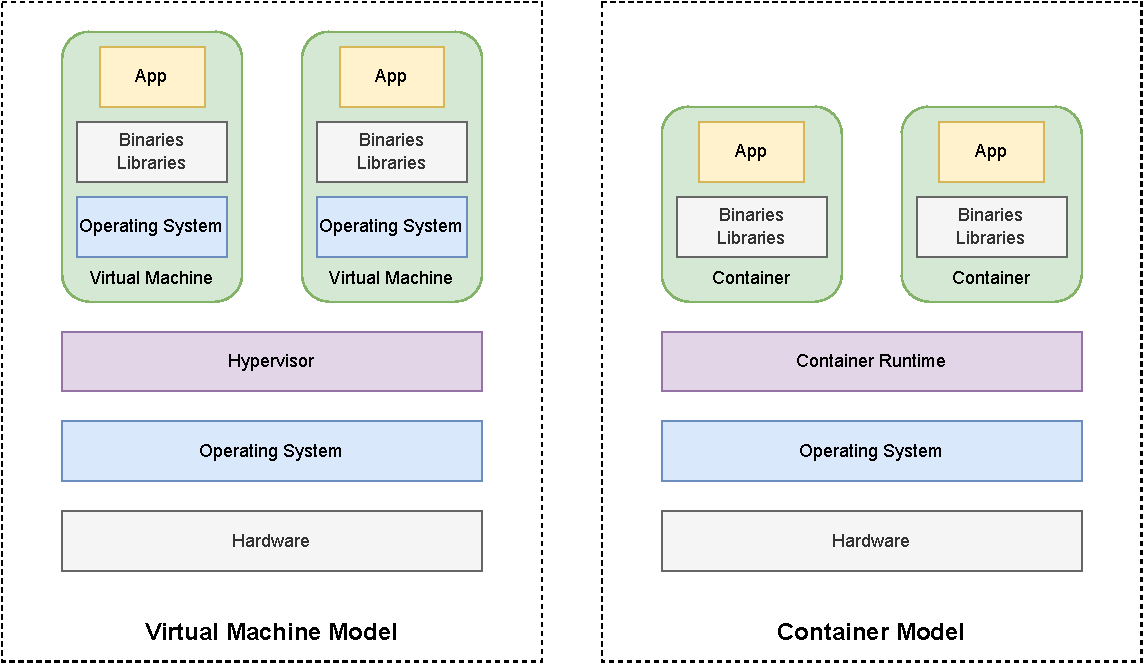
\includegraphics[width=.9\linewidth]{2_background/figures/vm-vs-container.pdf}

    \caption{Container and Virtual Machine based deployment models.}
    \label{fig:vm-vs-container}
\end{figure}

% Docker 
\Gls{docker} was introduced in Santa Clara at PyCon in 2013 \cite{pycon2013}. It jump started the revolution of \glspl{container} and was for many the first introduction to \gls{container} technologies. It was loved by developers for its portability and speed compared to traditional \gls{vm} deployments that were commonly used. Due to its immense popularity and praise, which it has managed to uphold according to recent surveys as conducted by stack overflow \cite{stack-overflow-survey}, \gls{docker} became the de facto standard in \gls{container} technologies and the similarly named company decided in 2015 to establish an open-source initiative that governs \gls{container} related standards \cite{open-container-standard}. Along with this they donated their container image specification format \cite{open-container-standard-image-spec} to this initiative as an open-source contribution. With this image specification standard in place, others could develop compatible container runtimes which were able to run the container images produced by said specification.

\section{A Shift in System Design}
\label{sec:background:soa}

% Small introduction an how it relates to prev chapter.
% Docker ->  Small deployment cost -> next level soa
In the previous section, we introduced \glspl{container} technology and \Gls{docker} (\cref{sec:background:containers}). These technologies reduced the cost of deployment by introducing a small, standardized unit of software. The adoption of container technology led to a shift in architectural design and led to an increase in usage of \glsfirst{soa} design patterns. Due to the little overhead in terms of system resources caused by the \gls{container} technology, it was an ideal candidate for independent self-contained components. This section will introduce the concept of a logical \textit{service} in distributed systems and documents the general trends caused by the shift in architectural paradigms.

% Before SOA, monoliths
\subsection{The Software Monolith}
\label{sec:background:soa:monolith}

\begin{figure}[!t]
    \centering
    
    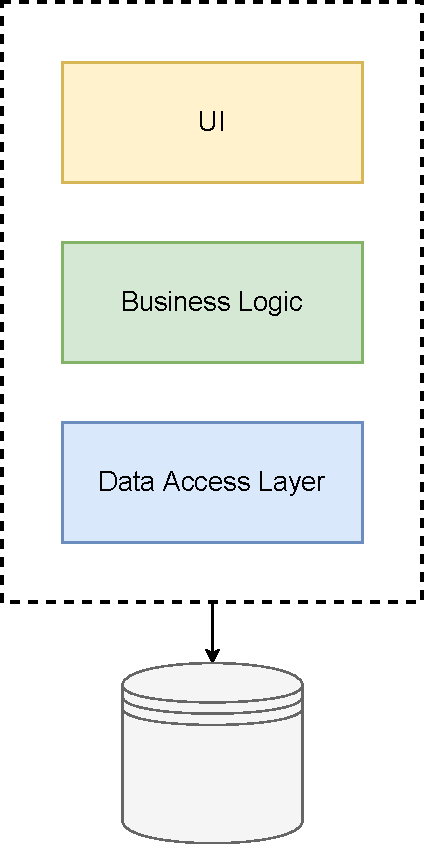
\includegraphics[width=0.3\linewidth]{2_background/figures/monolith-architecture.pdf}

    \caption[A monolithic software architecture]{A monolithic architecture. In this form of software design, all the software is contained into a single, self-contained software program depicted by the dashed line. }
    \label{fig:monolithic-architecture}
\end{figure}


Before the adoption of \gls{soa} principles and the notion of services in general, companies, and organizations alike used to create so-called software \glspl{monolith}. A monolithic approach in software design produces a self-contained software program where all of its dependencies, data access patterns and user interfacing components are combined (as depicted in \cref{fig:monolithic-architecture}). This makes monolithic architectures difficult to use in distributed systems without ad-hoc solutions or frameworks \cite{dragoni2017microservices}. A software \gls{monolith} can have several advantages, it produces a single binary, all code is colocated together,  and it is a battle-tested architecture. However, it can also have several disadvantages, it can be hard to maintain, codebases can become gigantic over time and lead to accumulated technical debt that makes the product unmaintainable with reasonable efforts \cite{fritzsch2018monolith}. This architectural pattern also forces the developers of the application to stick to their technical architecture, such as the choice of programming language and frameworks used. Furthermore, it can suffer from dependency hell, where updating or adding libraries can break existing systems  \cite{merkel2014docker}. Finally, the architecture does not scale very well, by scaling the application every single aspect or module has to be duplicated which is inefficient if only a subset of the application is put under load.



\subsection{A Service-Oriented Approach}
\label{sec:background:soa:service-oriented}


\begin{figure}[!t]
    \centering
    
    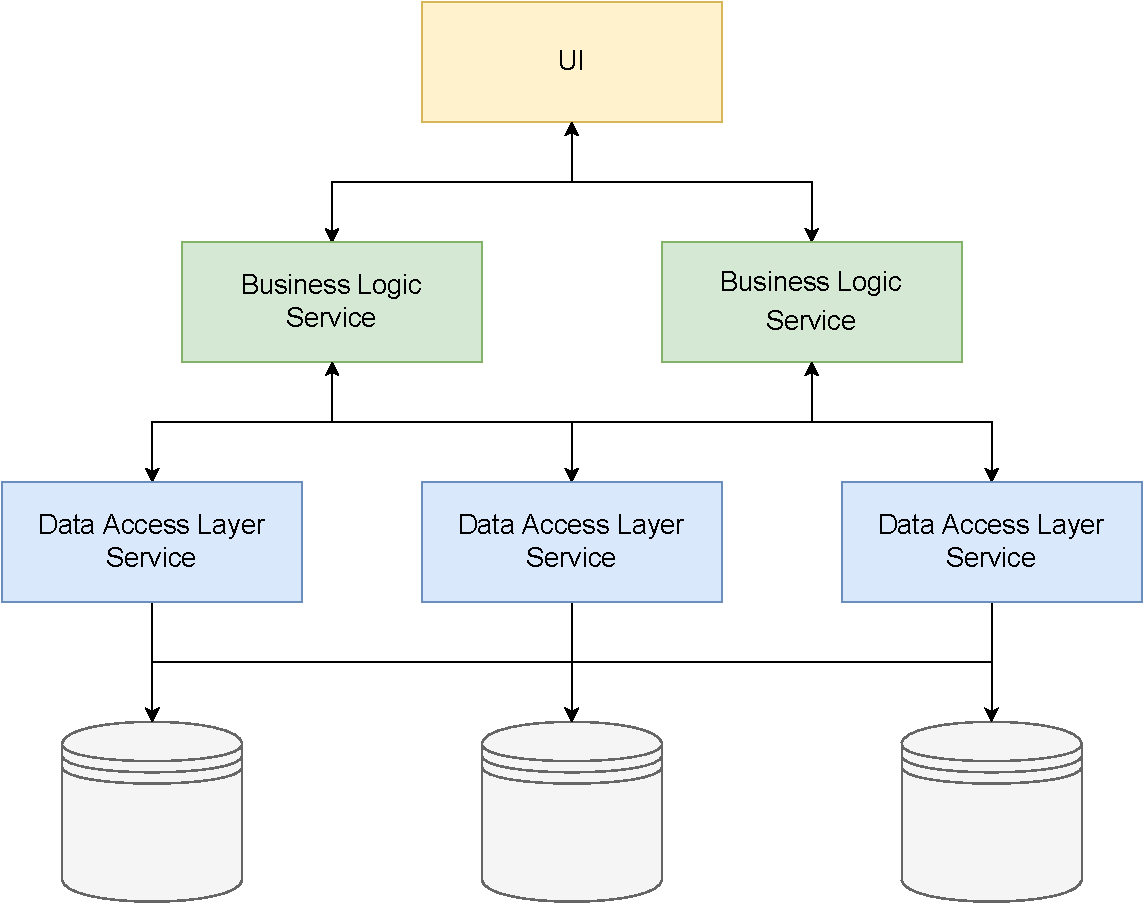
\includegraphics[width=.8\linewidth]{2_background/figures/service-oriented-architecture.pdf}

    \caption[A service-oriented software architecture]{A service-oriented approach. This architectural approach allows engineers to split applications into separate business components which enables them to scale and operate individually.}
    \label{fig:soa-architecture}
\end{figure}


% From monolith to SOA
% - Benefits
% - Microservices
As previously stated, the \gls{monolith}ic architecture was not well suited for use in distributed systems. This led to a newer style of software architectures that decomposed the business logic into  logical \textit{services}, where functionalities are encapsulated and abstracted from context \cite{perrey2003service}. This architectural paradigm meant that applications have to be decomposed into several self-contained units, which are then exposed via a \textit{service interface}. The service interface utilizes common communication standards so that it can be incorporated in new applications without much hassle \cite{ibm-soa}. Each service contains the code and data integrations required to execute a discrete business function. The core idea behind the \gls{soa} paradigm is that it promotes reusability and component sharing. This then translates into several benefits, such as an increase in scalability because it allows for scaling at a service level instead of having to scale an entire monolith. Furthermore, it allows software developers to use multiple technologies and frameworks, making it easier to pick the right tools for the job. This is enabled by the fact that services can exchange data over common protocols and agreed upon data representations, such as \gls{json} for example.


\subsection{Microservices}
\label{sec:background:soa:microservices}

% Intrdouce Microservices
% Small recap of why now

\begin{figure}[!t]
    \centering
    
    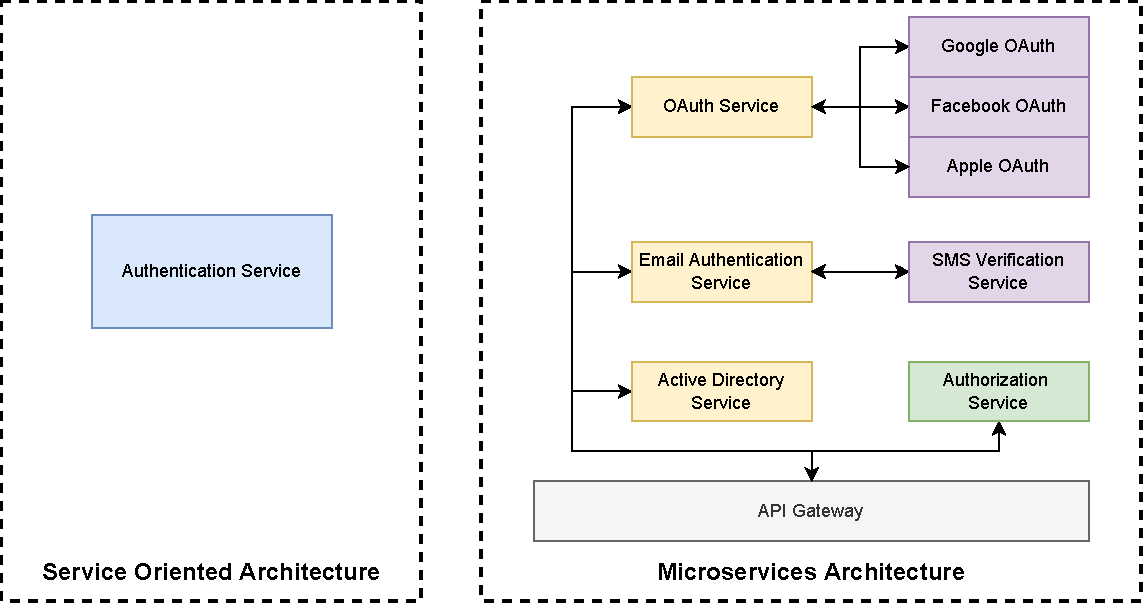
\includegraphics[width=.8\linewidth]{2_background/figures/microservices-vs-soa.pdf}

    \caption[The granularity of a microservices architecture]{Service-Oriented Architecture vs Microservices Architecture both  depicting an authentication service. Note: The granularity of the service definition depicts the most significant difference in the evolution of design.}
    \label{fig:soa-vs-microservices}
\end{figure}

The \textit{microservices} architecture (\cref{fig:soa-vs-microservices}) is an architectural style that emerged from the \gls{soa}. This evolvement was pushed by the  \gls{devops} movement and enabled by the decrease in deployment costs from the emerging \gls{container} technology \cite{amaral2015performance}.  The term \textit{microservice} dates in the context of distributed systems dates at least as far back as 2013 \cite{fowler-microservices}. It realizes its distinct itself from the \gls{soa}  paradigm by having a strong focus on its degree of independence regarding development and operation \cite{ibm-soa-vs-microservices}. The services that make up a \gls{soa}, can range from small, specialized services to enterprise-wide services, whereas a microservice consists of a highly specialized service, designed to do one thing well. This finer granularity allows for individual teams focussing on select subsets of an application and increases agility and development speed. However, this amplifies the problems that were mentioned above as it introduces more individual units in a complex system. Large companies such as Netflix that use such a microservices' architecture for example have reportedly managed to accumulate over 10000 microservices as of 2021 \cite{netflix-chaos, netflix-svc}.



\subsection{A New Set of Challenges}
\label{sec:background:soa:challenges}

% Down sides of a service oriented approach
% - Complexity
% - Network failures
% - Load balancing
% - Health cheecking
% - Serbice discovery
% Solutions to these complexitis
% - Fat clients
% - Enterprise Service Bus


\begin{figure}[!t]
    \centering
    
    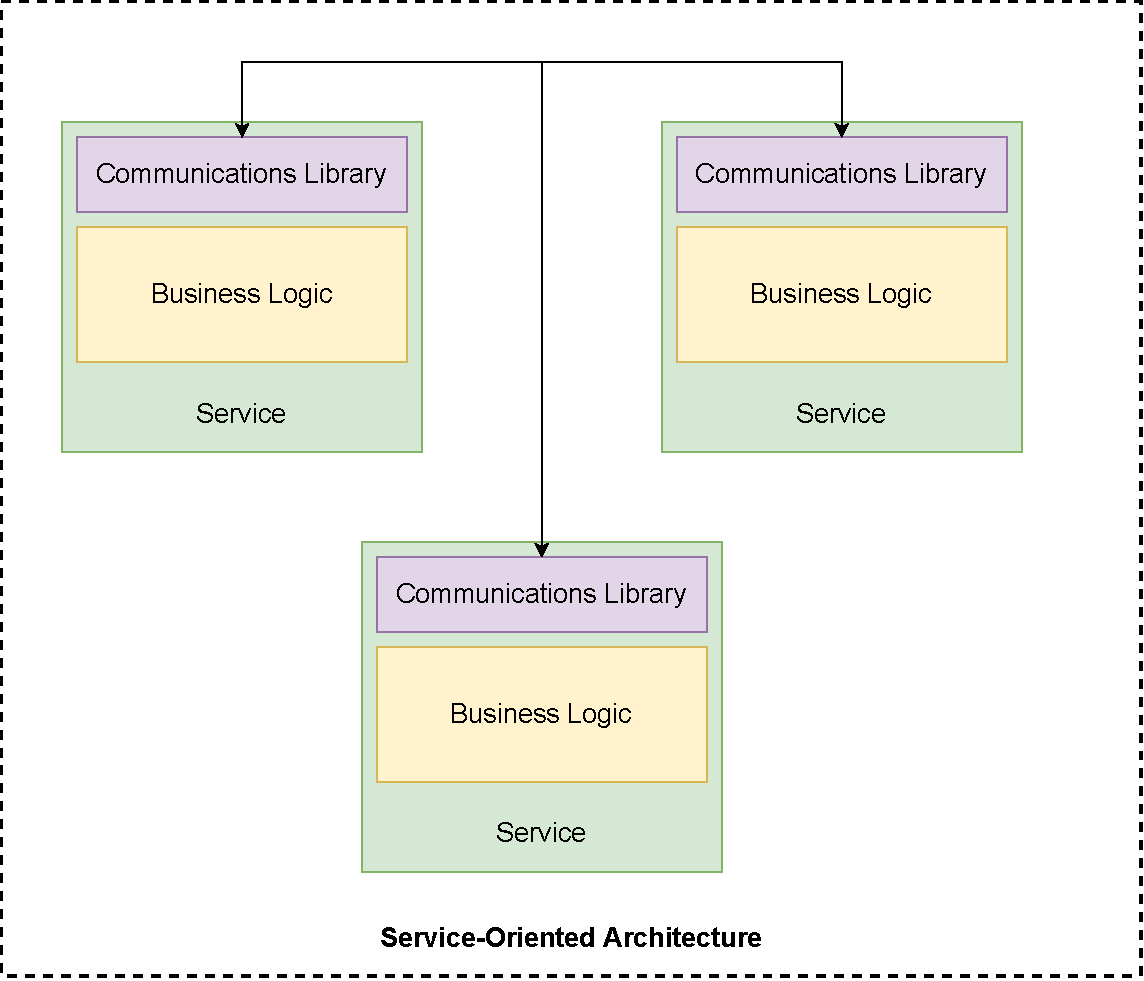
\includegraphics[width=.7\linewidth]{2_background/figures/software-lib-approach.pdf}

    \caption{Software library approach for solving the challenges introduces by a service-oriented design. In this design, the software library implements a uniform client and server API, designed to  handle fault tolerance, load balancing and latency optimizations to construct high-concurrency services.}
    \label{fig:software-lib-approach}
\end{figure}

However, by splitting the application up into several components, we introduce additional complexities. First off, the coarse granularity of the service-oriented design means that testing and validating every combination and condition may be very complex or even impossible \cite{mahmood2007service}. Furthermore, the loosely coupled services might be an architect's dream; however, it introduces additional complexities for a software developer \cite{fowler2012patterns}. Additionally, the service-to-service communications can now introduce failures, especially if they are carried out over unreliable networks such as the internet. Finally, the interoperability of services introduces additional challenges. How and where can we reach the services? Which version of the service is running and is it still compatible with everything? If there are multiple instances of this service, which one should be targetted to prevent overloading and ensure equal load? 



One approach used to solve these problems was through software libraries to handle all service-to-service communications (\cref{fig:software-lib-approach}) in a uniform way \cite{service-mesh-history}. Companies like Google, Netflix, and Twitter developed custom software libraries for this, such as Stubby \cite{stubby}, Hysterix \cite{hysterix} and Finagle \cite{finagle} respectively. These libraries would perform load balancing, implement retry mechanisms, routing, and telemetry. A downside of this approach was that this meant that the libraries were usually written in a single programming language, locking the developers in, or resulting in having to support multiple libraries. Furthermore, it resulted in a scenario where updating the library meant that every service implementing it also required an update. 

% \todo{double check ESB bit} Another approach used was to utilize another design pattern that implements an \gls{esb}, an open standards, message-based, distributed integration infrastructure that provides routing, invocation and mediation services to facilitate the interactions of disparate distributed applications and services in a secure and reliable manner \cite{menge2007enterprise}. This dedicated piece of infrastructure combines  Message-Oriented Middleware (MOM), web services, transformation and routing intelligence as a backbone for Service-Oriented Architecture.



\section{Kubernetes}
\label{sec:background:kubernetes}

In the previous sections we discussed the changes in deployment models (\cref{sec:background:containers}) and how this caused a shift in design based on decoupling business logic (\cref{sec:background:soa}). In this section, we introduce \gls{k8s}, a container-centric resource manager, that is the de facto standard within the field. With over 96\% of  organizations using or evaluating \gls{k8s} according to a recent survey \cite{cncf-survey-2021} conducted by the the \gls{cncf}, the industry-leading foundation for container technologies, it is clear that the technology had a large impact on the industry and technological developments around it. Throughout the remainder of the work presented in this thesis we use \gls{k8s}, as most of the systems we examine and evaluate, rely or build on top of \gls{k8s}. We also briefly introduce some relevant \gls{k8s} related concepts, which are used throughout this thesis, such as the architectural diagrams discussed in \cref{sec:survey:analysis:architectures}.

The \gls{k8s} project was initially conceived by Google and started in June 2014  and launched in early 2015 at OSCON \cite{kubernetes-launch}. It was designed to be a container-centric resource manager, and its design was heavily influenced by the internal tooling used within Google \cite{burns2016borg}. With the container as unit of compute, \gls{k8s} provides a streamlined approach to declaratively manage workloads. From \textit{service discovery} and \textit{load balancing} to \textit{storage orchestration}, \gls{k8s} aims to solve the many challenges that appear when managing large amounts of containers in production environments. Based on concepts of \textit{Control Theory} \cite{aastrom2021feedback, morris2010control}, the system uses a declarative approach which tries to keep the ecosystem in a desired state at any given time.

\Gls{k8s} consists of a set of components\footnote{\url{https://kubernetes.io/docs/concepts/overview/components/}} that have to be installed on several \textit{nodes}\footnote{\url{https://kubernetes.io/docs/concepts/architecture/nodes/}} (physical or \glspl{vm}) to form a compute \textit{cluster}. The core idea of \gls{k8s} is that is controlled through a centralized \textit{kube-apiserver}, which controls all components and acts as an interface for operators to control the cluster and manage workloads running on it.

\subsection{The Kubernetes Networking Model}
\label{sec:background:kubernetes:networking-model}

\Gls{k8s} relies on a specific networking model, which makes it easier for the \textit{cluster operator}\footnote{The term cluster operator is used throughout this thesis to indicate the person operating a Kubernetes cluster, i.e. deploying workloads, managing networking and security etc.} to manage and direct network traffic within the cluster. The networking model required essentially comes down to the following rules \cite{container-networking-from-scratch}.

\begin{enumerate}
  \item All containers can communicate with all other containers without \textit{NAT}
  \item All nodes can communicate with all containers (and vice-versa) without \textit{NAT}
  \item The IP that a container sees itself as is the same IP that others see it as
\end{enumerate}

\Gls{k8s} does not come with a solution that implements this networking model, however, it requires it for operation. There are many ways to implement the \gls{k8s} networking model, third-party solutions (often referred to as a \textit{Container Networking Interface}) such as \textit{Calico} or \textit{Flannel}. Another option commonly used to make use of \textit{Virtual Private Cloud} solutions offered by various cloud providers such as \gls{aws} or \gls{gcp}, which allow the user to emulate this flat networking model without having to install third-party software solutions.

\subsection{Pod}
\label{sec:background:kubernetes:pod}

Although \gls{k8s} is a container-centric resource manager, it does not use the container abstraction to manage the workloads within the ecosystem. Instead, it uses an abstraction on top of containers, namely the \gls{pod}. \Glspl{pod} are the smallest deployable units of computing that you can create and manage in Kubernetes\footnote{\url{https://kubernetes.io/docs/concepts/workloads/pods/}}. 

It consists of one or more containers that emulate a logical \textit{host}, much like a \gls{vm} would. This means that each \gls{pod} has its own isolated \textit{networking stack}\footnote{The networking stack, in the context of this thesis, refers to the Linux networking stack and consists of all the layers a packet has to traverse on a Linux-based system.} through \textit{namespaces} (\cref{sec:background:containers}), and that storage volumes are shared between containers inside a \gls{pod}. Networking between containers within the same \gls{pod} can be achieved through the \textit{loopback device} and reached through \textit{localhost} and there cannot be multiple processes that listen on the same port, much like a regular host. This is important to note, as this concept and network isolation paradigm is used by the most common \gls{sm} architecture discussed in this thesis (see \cref{sec:survey:analysis:architectures:per-service}).


\subsection{Service}
\label{sec:background:kubernetes:service}

The final \gls{k8s} concept we introduce is the notion of a \textit{service}\footnote{\url{https://kubernetes.io/docs/concepts/services-networking/service/}}. In \gls{k8s} the service abstraction provides a mechanism to expose an application as a network service. Briefly explained, it provides a stable IP address that is used to reach a set of \glspl{pod} allowing the cluster operator to expose those applications and provide a stable interface to reach them. 

Although we do use the \gls{k8s} service abstraction in this thesis during our experimental evaluation \cref{chap:experimental-evaluation}, it can cause some confusion since it conflicts with the definition of a logical service as explained in \cref{sec:background:soa}. Therefore, it is important to note that the term service refers to a \textit{logical service} in the context of this thesis and not to the \gls{k8s} concept with a similar name, unless specifically stated otherwise.
\section{Service Mesh}
\label{sec:background:service-mesh}

In the previous sections we discussed the evolution in deployment models (\cref{sec:background:containers}) and how this caused a shift in system design, based on decoupling business logic into logical services (\cref{sec:background:soa}). We then went on to briefly introduce \gls{k8s} and several related concepts (\cref{sec:background:soa}). In this section, we build on top of the topics discussed in the background chapter and introduce the \textit{\gls{sm} architecture}, which is at the core of the work presented in this thesis. It is an architectural style, that aims to solve the communicative challenges caused by service-oriented design.

% This section introduces a service mesh to the user
% What is a service mesh
% What does a service mesh try to solve
% Why is it becoming a thing now
% Is it a overhyped technology


\begin{figure}[!t]
    \centering
    
    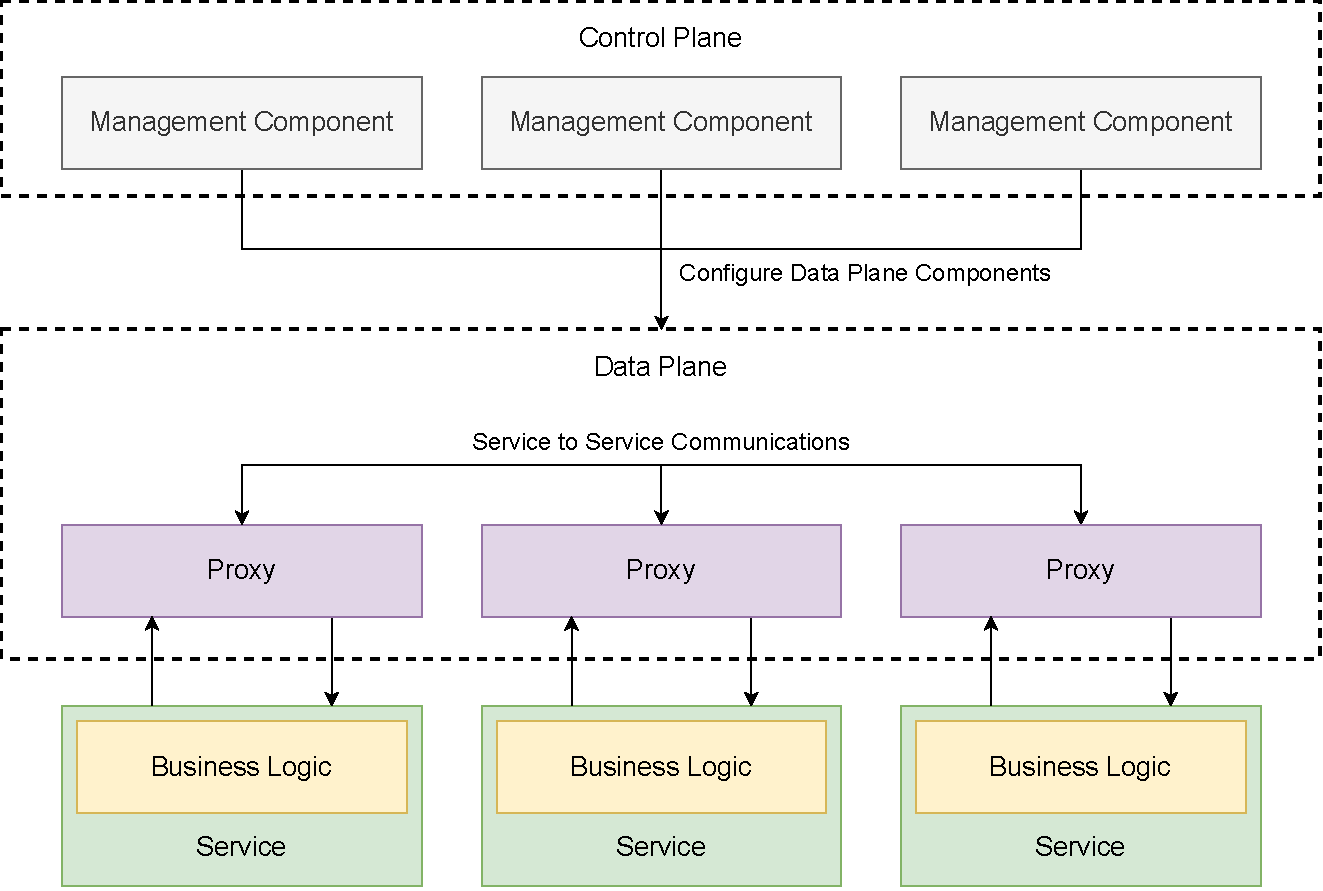
\includegraphics[width=\linewidth]{2_background/figures/service-mesh-architecture.pdf}

    \caption[\Gls{sm} architecture.]{\Gls{sm} architecture.}
    \label{fig:service-mesh-architecture}
\end{figure}

% Context
% Short intro service mesh, how it can add to latency/overhead
A \gls{sm} is a dedicated layer of networking infrastructure that sits between logical software services and aims to solve some communicative challenges introduces by a \gls{soa}. The terminology was introduced in the last decade \cite{service-mesh-manifesto}, and several systems adhering to this architecture have seen the light of day since. The premise of introducing additional observability in the system, increasing the reliability of it while also adding security best practices to little or no additional lines of application code made this technology a hot topic in the field. However, this technology does not come in the form of a zero cost offering. The \gls{sm} architecture introduces additional machinery to achieve its goals and is depicted in \cref{fig:service-mesh-architecture}. The components that make up a \gls{sm} can be divided into two  categories. A set of management components that constitute the \textit{Control Plane} and a set of components that handle the network traffic referred to as the \textit{Data Plane}.

\subsection{Data Plane}
\label{sec:background:service-mesh:data-plane}

The data plane is what actually defines the dedicated layer of networking infrastructure, it is what creates the mesh. It is created by placing \textit{proxies} in front of the logical services. The goal of these proxies is to intercept all traffic to and from a given service. All service-to-service communications, and direct requests to a service go through these proxies. Notably, these proxies are \textit{Layer 7-aware TCP proxies} like many popular general purpose proxies such as \textit{HAProxy}\footnote{\url{http://www.haproxy.org/}} or \textit{NGINX}\footnote{\url{https://www.nginx.com/}}. Although the choice of proxy is an implementation detail, most \gls{sm} use a proxy that has a focus on high performance and a feature set that aligns with the many benefits a \gls{sm} can provide (as discussed in \cref{sec:background:service-mesh:benefits}).

By introducing these proxies into the system, an increase in system resources is to be expected. More importantly, the introduction of a network proxy leads to an increase in the amount of network hops in the \textit{data path}\footnote{The term data path in this context, and throughout the rest of this thesis, refers to the machinery (both software and hardware) a network packet has to pass through to reach its destination.} for each packet. The downside of this is that this therefore leads to an increase in request latency and can cause for scalability concerns. In this thesis, we take an experimental approach to quantify the performance overheads caused by a \gls{sm} system. Therefore, we will focus on the impact of the data plane components.


\subsection{Control Plane}
\label{sec:background:service-mesh:control-plane}

A second set of components makes up the control plane of a \gls{sm} system. This set of components is used to manage and facilitate the functionalities of a \gls{sm}. It provides coordination and configuration for the data plane proxies and performs functions such as service discovery and metric aggregation. Another component often found in the control plane of \gls{sm} is a \textit{Certificate Authority}, which issues TLS certificates to the data plane proxies enabling them to authenticate each other and use encrypted communications. 

Compared to the data plane components, the control plane components have a lesser impact on the performance of systems. First, it does not affect the network traffic in the data path directly, and only has an impact on system resources. Furthermore, this impact is mostly static, as there often is just one instance of each component which provides a sharp contrast to the most common data plane design which results in a proxy per individual service (\cref{sec:survey:analysis:architectures:per-service}). 

\subsection{Benefits of a Service Mesh}
\label{sec:background:service-mesh:benefits}

To understand the benefits of a \gls{sm} system, we first need to understand which challenges such a system is trying to solve. As previously discussed in \cref{sec:background:soa}, we expanded on the benefits of a service-oriented approach, but also briefly explained some downsides of such an architecture. In short, it adds another layer of complexity into a system that comes in the form of communicative overhead. Services have to deal with the inherent by-products of communications and networking. Network connections can fail, services can crash or experience downtime, services now have to deal with load balancing and service discovery just to name a few of those challenges. 

The \gls{sm} architecture and the systems that implement this try to address these challenges in a uniform fashion. It provides a way to implement distributed systems best practices without having to modify the business logic that makes up a logical service. The advantages of a \gls{sm} architecture can be categorized into four groups.

\begin{enumerate}[leftmargin=3\parindent]
    \item \textbf{Observability}
    The first set of features and advantages related to a \gls{sm} system deals with the observability of communications. The data plane of a service mesh can log the details of network request in a uniform manner. Furthermore, it captures metrics such as request latencies, request payload sizes, request volumes, and status codes to name a few. Another desirable aspect is that it allows operators to view and create service topology maps, depicting the relations between services or inspect and trace individual requests throughout a system.
    
    \item \textbf{Reliability}
    Every engineer and user wants a reliable system; however, there are many challenges that one has to solve to make a system reliable. Network connections can fail, services can crash or experience downtime or a new software update can cause compatibility issues. A \gls{sm} tries to solve some of these problems by introducing a set of reliability features. Some of these include the ability to automate and configure request retries and timeouts. Another feature that helps in this area is the ability to perform traffic splitting and shifting, often used for \textit{canary deployment}\footnote{A  canary deployment is a software rollout strategy that is based on staged releases. The core idea is that the software is only available to a particular subset of users, which is slowly incremented over time. This practice serves as an early warning and can minimize the impact of failed deployments.}.

    \item \textbf{Security}
    A major advantage of using a \gls{sm} system is related to the security related features that it provides. One of the major challenges of modern IT systems is related to security and data privacy. How can we make sure that data cannot be observed by bad actors and limit or control the access within a system? Due to the design of the data plane all communications go through a network proxy (see \cref{sec:background:service-mesh:data-plane}). This enables a service mesh to automatically encrypt all data transfers in service-to-service communications through modern encryption standards. Furthermore, it enables the operator to configure access control for said services with finer granularity.
    
    \item \textbf{Programmability}
    A final category of features that a \gls{sm} provides is related to the programmability of such systems. The first set of programmability features is related to the type of proxy used in the data plane. Due to the layer 7 aware network proxies that it uses, it can make decisions based on application level protocol details. This allows an operator to configure networking, routing and load balancing on application level details such as \textit{HTTP} headers, paths or \textit{Kafka} topics. The second set of features that enable an additional layer of programmability is due to the extensibility features often found within the proxies used in \gls{sm} systems. Many of the popular data plane proxies such as \textit{Envoy} allow the user to extend the default feature set\footnote{\url{https://www.envoyproxy.io/docs/envoy/latest/extending/extending}}.

\end{enumerate}


\subsection{Alternatives to the Service Mesh Architecture}
\label{sec:background:service-mesh:alternatives}

We discussed the set of challenges that a \gls{sm} tries to solve, however, this set of challenges related to communications have existed long before the notion of a \gls{sm} even existed. How did we solve these challenges before, and what are some alternative solutions? 

One approach would be to manually configure and handle all the aspects and features that a \gls{sm} architecture implements. This would be the best performing option, requires no additional machinery to implement and allows the software engineers to use any language or framework, that best suit their needs to implement various logical services. The downside of this approach is that it will most likely lack in uniformity, and requires a significant effort from the software engineers to implement in a microservices architecture, as it would mean that engineers would have to manually manage and implement the intricacies of networking best practices and repeat the process for every single service.

Another approach used was to utilize another design pattern that implements an \textit{\gls{esb}}, an open standard, message-based, distributed integration infrastructure that provides routing, invocation and mediation services to facilitate the interactions of disparate distributed applications and services in a secure and reliable manner \cite{menge2007enterprise}. This dedicated piece of infrastructure combines  Message-Oriented Middleware, web services, transformation, and routing intelligence as a backbone for Service-Oriented Architecture. The most significant difference with the service mesh architecture, is that the services within such an \gls{esb} architecture relied on the infrastructure and middlewares of it \cite{samnewman2022}. In a \gls{sm} architecture, the services are not aware of any topology changes or that their networking traffic is being intercepted at all. This is a key difference and important to note, as it provides a clear separation of concerns from the \gls{esb} architecture frequently used in the 90s.

\begin{figure}[!t]
    \centering
    
    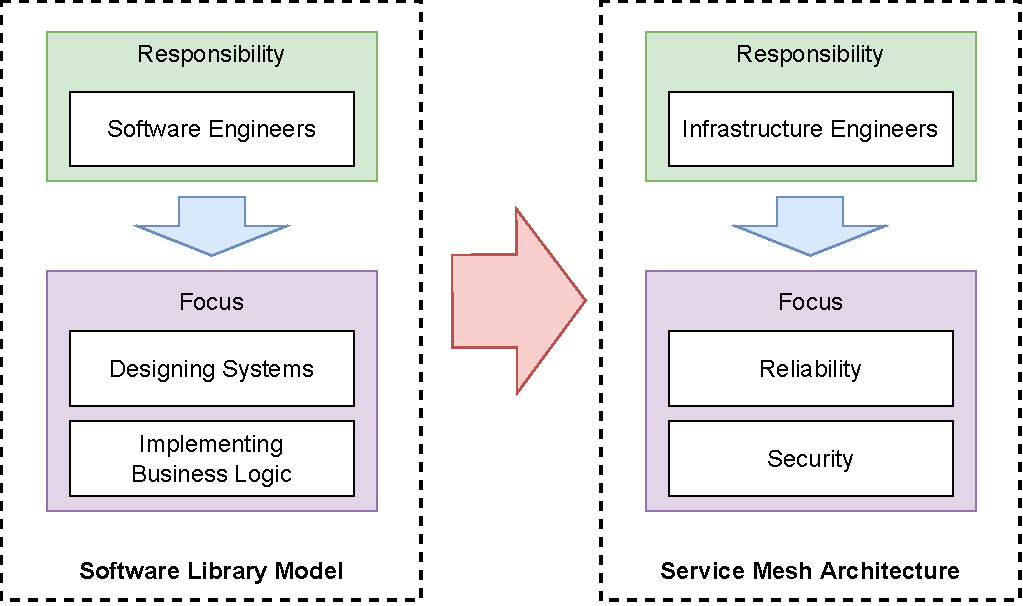
\includegraphics[width=0.8\linewidth]{2_background/figures/responsibility-model.pdf}

    \caption[\Gls{sm}responsibility model.]{\Gls{sm} responsibility model. Compares the shift in responsibilities compares to the software library approach and shows that it can provide a clear separation of concerns for the stakeholders involved. It allows the stakeholders involved to focus and work on the objectives that align with their roles.}
    \label{fig:service-mesh-responsibility-model}
\end{figure}

Another common alternative was already briefly touched upon in  \cref{sec:background:soa:challenges}, in which we introduced the software library-based approach that did not rely on additional machinery to be implemented. The software libraries are used to implement a uniform client and server interface. With a focus on load balancing mechanisms, fault tolerance with retry and timeout feature sets the software library implements many of the features and mechanisms present in a \gls{sm} system. This approach can be the most performant option, as it does not introduce additional network hops and complex systems. However, a clear downside of such an approach is that this would mean that software engineers would be limited to use a single programming language to implement all business logic, or maintain multiple software libraries to support different technology stacks. Furthermore, an update to such a library would mean that all the services running that library would require an update as well. 

In \cref{fig:service-mesh-responsibility-model} we compare the most common alternative to the \gls{sm} architecture and shows the shift in responsibility that it caused. By using a \gls{sm} architecture, the infrastructure engineers maintain the \gls{sm} system. The features that a \gls{sm} provides align with the goals and objectives that such a stakeholder has, such as maintaining a reliable platform and having a security-first mindset. For software engineers this meant that they do not have to maintain, update and implement these libraries and can focus on system design and implementing business logic instead. This provides a clear separation of concerns and allows the stakeholders to focus more on the goals and objectives aligned with their respective roles.
\section{Cloud Native Computing Foundation}
\label{sec:background:cncf}

% Explain the CNCF
% - What are the goals of the CNCF
% - Well established  entity and governing body in the field

In this section, we briefly introduce the \glsfirst{cncf}, an entity that is often mentioned throughout this thesis as they are a governing body in the field. 

The \gls{cncf} is part of the \textit{Linux Foundation}\footnote{The Linux Foundation  is a non-profit technology consortium that aims to standardize Linux, support its growth, and promote its commercial adoption.} and was founded in 2015 at the same time the first version of \gls{k8s} was introduced. The goal of this foundation is to be an open-source, vendor-neutral \todo{check this ref, literal citation from the website} hub of \textit{cloud native computing} \cite{cncf-charter}. Where cloud native technologies are defined as technologies that \say{...empower organizations to build and run scalable applications in modern, dynamic environments such as public, private, and hybrid clouds. Containers, service meshes, microservices, immutable infrastructure, and declarative APIs exemplify this approach}.

The \gls{cncf} governs many open-source software projects, \gls{k8s} is one of such projects as it was donated to the foundation upon release. There are currently 1119 projects governed by the foundation at the time of writing, which together, form the \textit{CNCF landscape}. This landscape (as seen in the Appendix, \cref{appendix:cncf-landscape}) has an estimated market cap of \$20.3 trillion and a total funding of \$51.6 billion\footnote{\url{https://landscape.cncf.io/}}. Projects are categorized in three levels of maturity\footnote{\url{https://www.cncf.io/projects/}}, ranging from (in ascending order) \textit{Sandbox}, to \textit{Incubated} to \textit{Graduated}.

Throughout the rest of this thesis, we use several projects that are governed by the \gls{cncf}, as many of the \gls{sm} systems are part of the landscape. In addition to that, we use \gls{k8s} as the resource manager to construct our experimental environment (see \cref{sec:experiments:design:environment:cluster}) and use various other projects in our implementation of \textit{Mesh Bench} (see \cref{sec:system:implementation}). In addition to the projects, we use a lot of the data the foundation gathers through their annual surveys, which provide key insights into the field of cloud native, and serverless technologies.
 


